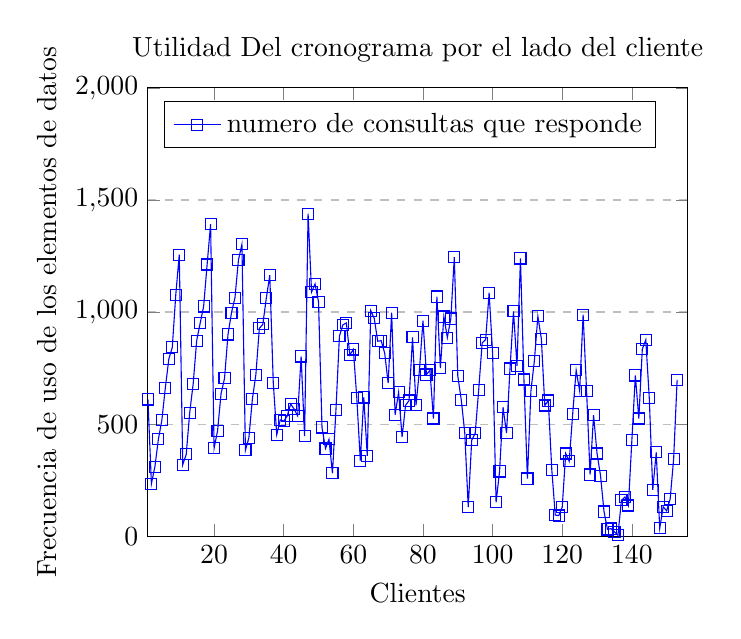
\begin{tikzpicture}
\begin{axis}[
    title={Utilidad Del cronograma por el lado del cliente},
    xlabel={Clientes},
    ylabel={Frecuencia de uso de los elementos de datos},
    xmin=1, xmax=156,
    ymin=0, ymax=2000,
    xtick={},
    ytick={},
    legend pos=north west,
    ymajorgrids=true,
    grid style=dashed,
]

\addplot[
    color=blue,
    mark=square,
    ]
    coordinates {
    %USO EXACTO
    (1,610)
(2,234)
(3,310)
(4,432)
(5,517)
(6,662)
(7,790)
(8,843)
(9,1077)
(10,1256)
(11,319)
(12,365)
(13,551)
(14,680)
(15,872)
(16,950)
(17,1025)
(18,1212)
(19,1392)
(20,392)
(21,470)
(22,635)
(23,704)
(24,900)
(25,997)
(26,1064)
(27,1232)
(28,1302)
(29,383)
(30,439)
(31,612)
(32,720)
(33,927)
(34,945)
(35,1062)
(36,1164)
(37,685)
(38,453)
(39,519)
(40,513)
(41,536)
(42,590)
(43,567)
(44,537)
(45,802)
(46,446)
(47,1439)
(48,1089)
(49,1125)
(50,1046)
(51,485)
(52,391)
(53,432)
(54,281)
(55,562)
(56,892)
(57,943)
(58,951)
(59,809)
(60,833)
(61,616)
(62,337)
(63,619)
(64,358)
(65,1006)
(66,972)
(67,870)
(68,872)
(69,817)
(70,683)
(71,997)
(72,541)
(73,642)
(74,443)
(75,584)
(76,605)
(77,887)
(78,584)
(79,743)
(80,961)
(81,721)
(82,740)
(83,525)
(84,1069)
(85,750)
(86,980)
(87,886)
(88,971)
(89,1245)
(90,715)
(91,608)
(92,462)
(93,130)
(94,428)
(95,459)
(96,652)
(97,862)
(98,877)
(99,1086)
(100,817)
(101,151)
(102,289)
(103,575)
(104,460)
(105,748)
(106,1003)
(107,760)
(108,1239)
(109,699)
(110,257)
(111,647)
(112,783)
(113,981)
(114,881)
(115,583)
(116,605)
(117,297)
(118,94)
(119,92)
(120,130)
(121,369)
(122,334)
(123,545)
(124,740)
(125,648)
(126,988)
(127,646)
(128,275)
(129,540)
(130,369)
(131,270)
(132,110)
(133,30)
(134,34)
(135,19)
(136,4)
(137,160)
(138,175)
(139,137)
(140,428)
(141,717)
(142,525)
(143,835)
(144,876)
(145,617)
(146,207)
(147,374)
(148,35)
(149,131)
(150,113)
(151,166)
(152,345)
(153,697)
    };
    \legend{numero de consultas que responde}

\end{axis}
\end{tikzpicture}

